\begin{definition}{Réseaux Bayésiens}{bayesianNetworks}
    Un réseau bayésien est un graphe orienté acyclique (DAG) dont les nœuds représentent des variables aléatoires et les arcs représentent des dépendances conditionnelles.\\
    Ils permettent de représenter des distributions de probabilités conjointes de manière compacte, de construire des modèles de raisonnement probabiliste et de faire de l'inférence.
    \begin{itemize}
        \item Les nœuds représentent des variables aléatoires
        \item Les arcs représentent des dépendances (\textit{causilités?}) conditionnelles ainsi que des distributions de probabilités pour chaque variable aléatoire \textbf{étant donné} ses parents
        % \item Les nœuds sont associés à des probabilités conditionnelles
    \end{itemize}
    Façon compacte de représenter des \textbf{probabilités conjointes}.
    
\end{definition}

% \begin{example}\leavevmode
%     \begin{figure}[H]
%         \centering
%         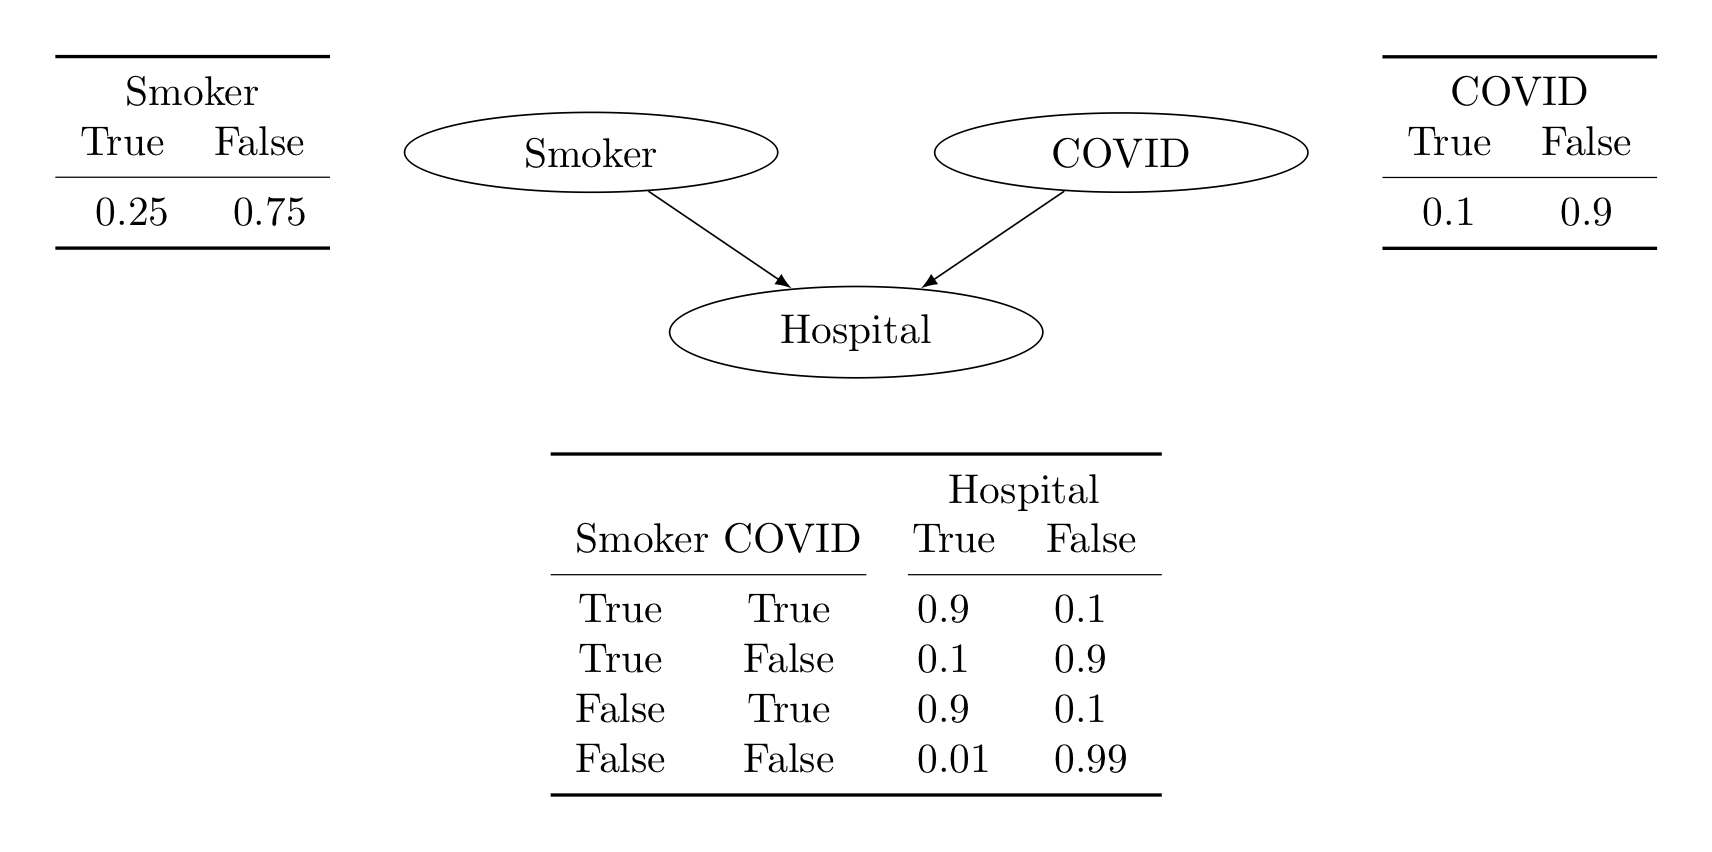
\includegraphics[width=0.6\linewidth]{pictures/bayesianNetwork.png}
%         \caption{Réseau bayésien}
%         \label{fig:bayesianNetwork}
%     \end{figure}
% \end{example}

La topologie du \textbf{RB} modélise les relations d'influence entre les variables aléatoires. 

Un arc $X \rightarrow Y$ signifie que $X$ influence $Y$.

Si $X$ n'a pas de parents, alors sa distribution de probabilité est dite \textbf{inconditionnelle} ou \textbf{à priori}.
Si $X$ a des parents, alors sa distribution de probabilité est dite \textbf{conditionnelle} ou \textbf{à posteriori}.
Chaque nœuds est associé à une table de probabilités conditionnelles (CPT) qui spécifie la probabilité de chaque valeur de la variable aléatoire étant donné les valeurs de ses parents. 




\begin{example}\leavevmode
    Voici un exemple du livre \textit{Artificial Intelligence: A Modern Approach} de Stuart Russel et Peter Norvig. 
    Considérons la situation suivante: 
    \begin{itemize}
        \item Je suis au travail et mes voisins Marie et John m'ont promis de \textbf{m'appeller} chaque fois que mon \textbf{alarme} se déclenche.
        \item \textbf{Jean m'appelle} pour me dire que mon alarme s'est déclenchée. 
            \begin{itemize}
                \item Cependant, il \textbf{la confond } parfois avec la sonnerie du téléphone
            \end{itemize}
        \item \textbf{Marie m'appelle pas toujours} 
            \begin{itemize}
                \item Elle écoute de la musique et ne l'entend pas toujours
            \end{itemize}
        \item Mon alarme peut également sonner à cause de \textbf{séismes}. 
        \item $\longrightarrow$ \textbf{Comment conclure qu'il y a un cambriolage?}
    \end{itemize}
    On représente cette situation par le réseau bayésien suivant: 
    % construit le graphe avec tikz
    \begin{figure}[H]
    \centering
    \scalebox{0.8}{
        \begin{minipage}{0.45\textwidth}
            \begin{tikzpicture}
              % Dessinez les nœuds du graphe
                \node[state] (0) at (0,0) {Alarme};
                \node[state] (1) [above right =of 0] {Séisme};
                \node[state] (2) [above left =of 0] {Combriolage};
                \node[state] (3) [below right =of 0] {MarieAppelle};
                \node[state] (4) [below left =of 3] {JeanAppelle};
                
                \path (2) edge[arrow] (0);
                % \path (1) edge[arrow][loop above] (1);
                \path (1) edge[arrow] (0);
                \path (0) edge[arrow] (3);
                \path (0) edge[arrow] (4);
            \end{tikzpicture}
            \caption{Réseau bayésien de l'exemple}
            \label{fig:graph1}
        \end{minipage}
    }
    \end{figure}
    Voici les probabilités conditionnelles associées à ce réseau bayésien: 
    \begin{figure}[H]
        \centering
        \scalebox{0.8}{
            \begin{minipage}{0.45\textwidth}
                \begin{tabular}{|c|c|}
                    \hline
                    $P(Combriolage)$ & $P(\neg Combriolage)$ \\
                    \hline
                    0.001 & 0.999 \\
                    \hline
                \end{tabular}
                \caption{Probabilités de $Combriolage$}
                \label{fig:graph1}
            \end{minipage}
            \begin{minipage}{0.45\textwidth}
                \begin{tabular}{|c|c|}
                    \hline
                    $P(Séisme)$ & $P(\neg Séisme)$ \\
                    \hline
                    0.002 & 0.998 \\ 
                    \hline
                \end{tabular}
                \caption{Table des probabilités de $Séisme$}
                \label{fig:graph1}
            \end{minipage}
        } 

        \scalebox{0.8}{
            \begin{minipage}{0.45\textwidth}
                \begin{tabular}{|c|c|c|}
                    \hline
                    $Combriolage$ & $Séisme$ & $P(Alarme)$ \\
                    \hline
                    $V$ & $V$ & 0.95 \\ 
                    $V$ & $F$ & 0.94 \\ 
                    $F$ & $V$ & 0.29 \\ 
                    $F$ & $F$ & 0.001 \\
                    \hline
                \end{tabular}
                \caption{Table des probabilités conditionnelles de $Alarme$}
                \label{fig:graph1}
            \end{minipage}
        } 

        \scalebox{0.8}{
            \begin{minipage}{0.45\textwidth}
                \begin{tabular}{|c|c|}
                    \hline
                    $Alarme$ & $P(JeanAppelle)$ \\
                    \hline
                    $V$ & 0.90 \\
                    $F$ & 0.05 \\
                    \hline
                \end{tabular}
                \caption{Table des probabilités conditionnelles de $JeanAppelle$}
                \label{fig:graph1}
            \end{minipage}
            \begin{minipage}{0.45\textwidth}
                \begin{tabular}{|c|c|}
                    \hline
                    $Alarme$ & $P(MarieAppelle)$ \\
                    \hline
                    $V$ & 0.70 \\
                    $F$ & 0.01 \\
                    \hline
                \end{tabular}
                \caption{Table des probabilités conditionnelles de $MarieAppelle$}
                \label{fig:graph1}
            \end{minipage}
        } 
    \end{figure}

\end{example}

\begin{note}
    Les réseaux bayésiens peuvent avoir des variables aléatoires continues ou discrètes.

    Les arcs entre les noeuds peuvent représenter une relation de causalité comme par exemple. 
    $Rain \rightarrow Traffic$ signifie que Rain cause Traffic.
    Cependant, ce n'est pas toujours le cas. De manière générale, les arcs représentent des dépendances conditionnelles. 
    Cela signifie que si on connait la valeur des parents d'un noeuds, alors on peut déduire la valeur du noeud et le reste n'a pas d'importance.
\end{note}

Nous savons que par définition, $P(A,B) = P(A|B)P(B)$.
Nous pouvons donc écrire la probabilité conjointe d'un réseau bayésien comme suit: 
\begin{equation}
    P(X_1, X_2, \dots, X_n) = \prod_{i=1}^{n} P(X_i | Parents(X_i)) 
\end{equation} 
Où $Parents(X_i)$ est l'ensemble des parents directe de $X_i$ dans le réseau bayésien.

\begin{example}\leavevmode
    En utilisant le réseau bayésien de l'exemple précédent, nous pouvons calculer la probabilité conjointe de toutes les variables aléatoires comme suit: 
    \begin{align*}
        P(C=F, S=F, A=V, J=V, M=V) 
        &= P(C=F)P(S=F)P(A=V|C=F, S=F)\\ & P(J=V|A=V)P(M=V|A=V) \\
        &= 0.999 \times 0.998 \times 0.001 \times 0.90 \times 0.70 \\
        &= 0.000628
    \end{align*}
\end{example}

Pour calculer les probabilités marginales, on peut ignorer les noeuds 
\textbf{dont les descendants ne sont pas les noeuds observés}

\begin{example}\leavevmode
    \begin{align*}
        P(C=F \cap A=V) &= \sum_{s} \sum_{j} \sum_{m} P(C=F, S=s, A=V, J=j, M=m) \\
                        &= \sum_{s} P(A=V | C=f, s) P(C=F) P(S=s) 
    \end{align*}
    On peut ignorer $J$ et $M$ car ils ne sont pas des descendants de $C$ qui est observé.
    Cependant, on ne peut pas ignorer $S$ car A est un descendant de $S$ et $A$ est observé.
\end{example}

\subsection{Inférence} % (fold)
\label{sub:inference}

\subsubsection{Inférence par énumeration} % (fold)
\label{sec:enumeration}


\begin{remark}\leavevmode
    N'importe quelles probabilités peuvent être utiliser à partir de la distribution de probabilités conjointes.
    \begin{align*}
        P(B | j, m) &= \alpha \sum_{e,a} P(B, e, a, j, m) \\ 
                    &= \alpha \sum_{e,a} P(B) P(e) P(a|B,e) P(j|a) P(m|a) \\
    \end{align*}
    Où $\alpha$ est une constante de normalisation. C'est comme si on marginalisait sur toutes les variables aléatoires sauf $B$ qui est la variable aléatoire dont on veut calculer la probabilité.

    Le problème est que le nombre de calculs à effectuer est exponentiel en fonction du nombre de variables aléatoires.
\end{remark}

Voici la procèdure pour calculer une probabilité marginale avec l'inférence par énumération: 

\begin{enumerate}
    \item \textbf{Initiliasation}: Toutes les tables de probabilités conditionnelles sont les facteurs initiaux.
    \scalebox{0.8}{
        \begin{minipage}{0.45\textwidth}
            \begin{tikzpicture}
              % Dessinez les nœuds du graphe
                \node[state] (0) at (0,0) {Rain};
                \node[state] (1) [right =of 0] {Traffic};
                \node[state] (2) [right =of 1] {Late for work};
                \path (0) edge[arrow] (1);
                \path (1) edge[arrow] (2);
            \end{tikzpicture}
            \label{fig:graph2}
            
        \end{minipage}
        % \caption{Réseau bayésien de l'exemple}
        }
        
    Les probabilités conditionnelles associées à ce réseau bayésien: 
    \begin{table}[H]
        \centering
        \begin{tabular}{|ll|}
            \hline
            $P(Rain)$ & $P(\neg Rain)$ \\ 
            \hline 
            0.1 & 0.9 \\
            \hline 
        \end{tabular}
        \caption{Tableau des probabilités de $P(R)$}
    \end{table}

    \begin{table}[H]
        \centering
        \begin{tabular}{|l|l|l|}
            \hline
            $Rain$ & $Traffic$ & 0.8 \\ 
            $Rain$ & $\neg Traffic$ & 0.2 \\
            $\neg Rain$ & $Traffic$ & 0.1 \\
            $\neg Rain$ & $\neg Traffic$ & 0.9 \\
            \hline
        \end{tabular}
        \caption{Tableau des probabilités conditionnelles de $P(T | R)$}
    \end{table}

    \begin{table}[H]
        \centering
        \begin{tabular}{|l|l|l|}
            \hline
            $Traffic$ & $Late$ & 0.3 \\ 
            $Traffic$ & $\neg Late$ & 0.7 \\
            $\neg Traffic$ & $Late$ & 0.1 \\
            $\neg Traffic$ & $\neg Late$ & 0.9 \\
            \hline
        \end{tabular}
        \caption{Tableau des probabilités conditionnelles de $P(L | T)$}
        \label{tabl:late}
    \end{table}
    Pour calculer $P(Late)$, on doit calculer la probabilité conjointe de toutes les variables aléatoires. 
    \begin{align*}
        P(Late) &= \sum_{r, t} P(r, t, L) \\
                &=\sum_{r,t} P(r) P(t|r) P(l|t) \\
    \end{align*}

    \begin{remark}\leavevmode
        Si $Late$ avait la valeur observée $Vrai$, alors  dans le tableau \ref{tabl:late}, on ne considère que les lignes où $Late$ est vrai.
    \end{remark}

    \item \textbf{Propagation/Join}: On propage les facteurs en multipliant les facteurs qui ont des variables en commun. C'est comme si on faisait une jointure sur les variables en commun. Même idée si on doit faire un join avec +2 variables.
        Par exemple, pour \textbf{join} $R$, on a $P(R) \times P(T | R) \implies P(R, T)$.
        la table de probabilités conditionnelles de $P(R, T)$ est: 
        \begin{table}[H]
            \centering
            \begin{tabular}{|l|l|l|}
                \hline
                $R$ & $T$ & 0.08 $= 0.1 \cdot 0.8$ \\ 
                $R$ & $\neg T$ & 0.02 $= 0.1 \cdot 0.02$\\
                $\neg R$ & $T$ & 0.09 $= 0.9 \cdot 0.1$\\
                $\neg R$ & $\neg T$ & 0.81 \\
                \hline
            \end{tabular}
            \caption{Tableau des probabilités conditionnelles de $P(R, T)$}
            \label{tab:rt}
        \end{table}
    \item \textbf{Elimination}: On élimine les variables qui ne sont pas observées en sommant les facteurs qui ont les mêmes variables. 
        Attention à ne pas supprier les variables qui sont observées ou bien celle qui nous intéresse.
        On élimine jusqu'a ce qu'il nous reste que la variable dont on veut calculer la probabilité.
        La table \ref{tab:rt} devient, lorsque on élimine $R$:
        \begin{table}[H]
            \centering
            \begin{tabular}{|l|l|}
                \hline
                $T$ & 0.17 \\ 
                $\neg T$ & 0.83 \\
                \hline
            \end{tabular}
            \caption{Tableau des probabilités conditionnelles de $P(T)$}
            \label{tab:t}
        \end{table}
        On a additionné les lignes ou $T$ avait la même valeur car nous voulons supprimer $R$.


\end{enumerate}



\subsubsubsection{Elimination de variables} % (fold)

L'idée est de réduire le nombre de calculs à effectuer en déplaçant les sommes vers l'intérieure de l'équation.
\begin{align*}
    P(B | j, m) &= \alpha \sum_{e,a} P(B) P(e) P(a|B,e) P(j|a) P(m|a) \\
                &= \alpha P(B) \sum_{e} P(e) \sum_{a} P(a|B,e) P(j|a) P(m|a) \\
\end{align*}
De cette manière on élimine les variables qui sont répétées dans les sommes.



L'idée est de marginaliser (éliminer) le plut tôt possible une variable (qui n'est pas utile). 

\warningbox{
    Tu ne peux marginaliser une variable tant que tu n'as pas join les facteurs qui ont la variables en commun.
}

\begin{figure}[H]
    \begin{center}
        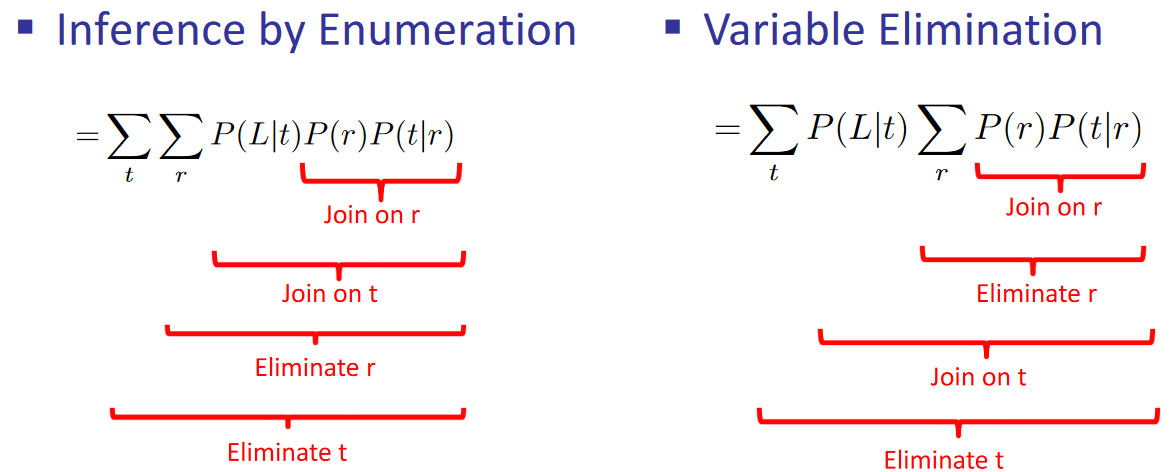
\includegraphics[width=0.4\textwidth]{pictures/ve.png}
    \end{center}
    \caption{Enumératin vs VE}\label{fig:ve}
\end{figure}

Si il y a des variables observée. Lors des jointures, on ne considère que les lignes où les variables observées ont la valeur observée.
Lorsqu'a la fin, il ne reste que la variable dont on veut calculer la probabilité ainsi que les variables observées, 
on normalise le résultat en divisant par la somme des probabilités.

\begin{figure}[H]
    \begin{center}
        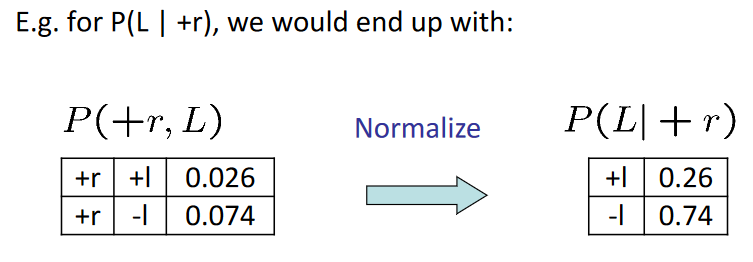
\includegraphics[width=0.4\textwidth]{pictures/veevidence.png}
        \hspace{1cm}
        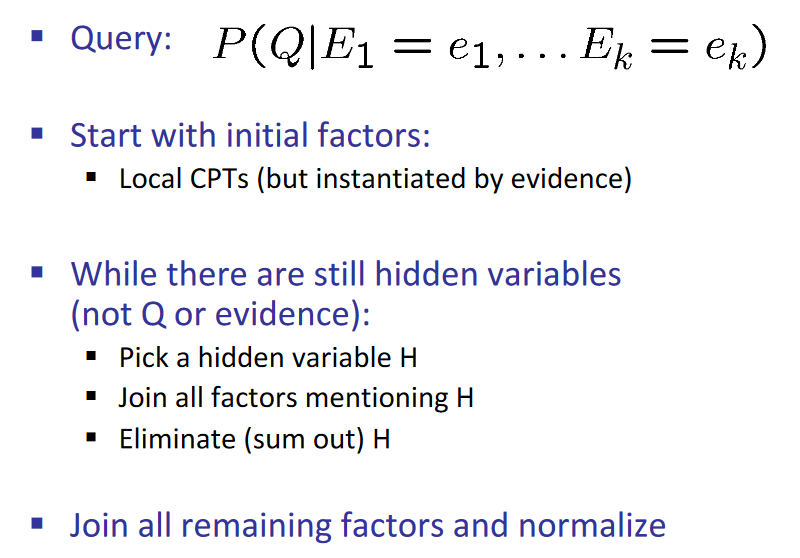
\includegraphics[width=0.4\textwidth]{pictures/vealgo.png}
    \end{center}
    \caption{VE avec evidence + algo}\label{fig:veevidence}
\end{figure}

\begin{remark}\leavevmode
    $P(B | j, m) = \propto P(B, j, m)$
    Cela signifie que l'on peut calculer la probabilité conditionnelle en calculant la probabilité conjointe.
    Il suffit ensuite de normaliser le résultat en divisant par la somme des probabilités.
\end{remark}


\subsection{D-Separation} % (fold)
\label{sub:d_separation}

\begin{definition}{D-Séparation}{d-separation}
    La D-séparation dans un réseau bayésien est un outil pour déterminer l'indépendance conditionnelle.
    entre des ensembles de variables en analysant les chemins entre ces variables dans le graphe du réseau bayésien
    Elle est basée sur la notion de \textbf{triplet actif} et \textbf{triplet inactif} qui forment un chemin \textbf{actif} ou \textbf{inactif}.
    \begin{itemize}
        \item \textbf{Chemin} : Un chemin entre deux nœuds A et B dans un réseau bayésien est une séquence de liens qui connectent ces deux nœuds. Il est divisé en \textbf{triplets} et n'est pas dirigé.
        \item \textbf{Chemin Actif}:  Un chemin est actif s'il n'est pas bloqué par des triplets inactifs. Il peut transmettre l'information entre les nœuds A et B.
        \item \textbf{Chemin Inactif}: Un chemin est inactif s'il contient un ou plusieur triplets inactifs. Il ne peut pas transmettre l'information entre les nœuds A et B.
        % \item \textbf{Blocage} : Un chemin peut être bloqué par l'une des trois conditions suivantes :
            % \begin{enumerate}
                % \item S'il y a un ou plusieurs triplets actifs dans le chemin, alors les noeuds des extrémités ne sont pas indépendants conditionnellement.
                % \item Si tous les chemins entre les noeuds des extrémités sont bloqués, alors les noeuds des extrémités sont indépendants conditionnellement.
            % \end{enumerate}
    \end{itemize}
\end{definition}

% Pour savoir si un Triplet est actif ou inactif, il faut regarder les noeuds qui le composent. 
\begin{figure}[H]
    \begin{center}
        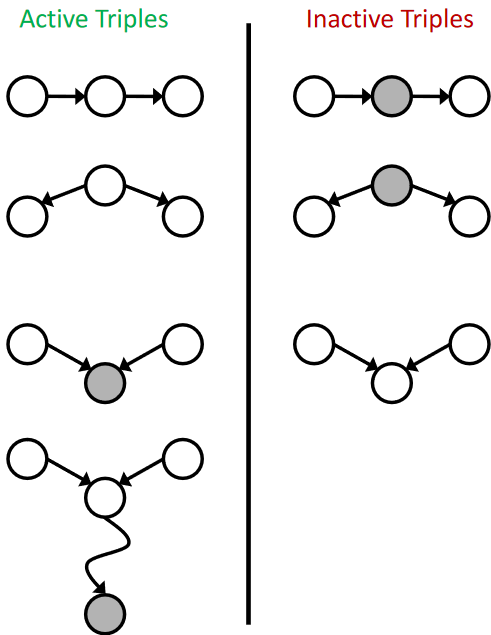
\includegraphics[width=0.3\textwidth]{pictures/triplet.png}
    \end{center}
    \caption{Table pour savoir si un triplet est actif ou pas}\label{fig:triplet}
\end{figure}

\begin{remark}\leavevmode
    Cette technique est utile pour savoir si deux variables aléatoires sont indépendantes conditionnellement. 
    Il n'est pas toujours facile, lors du design du réseau bayésien, de savoir quelles variables aléatoires sont indépendantes conditionnellement.
\end{remark}

% subsection D-Separation (end)

\subsection{Echantillonage} % (fold)
\label{sub:echantillonage}

\subsubsection{Prior} % (fold)
\label{sec:prior}

\begin{remark}\leavevmode
    L'inférence par énumération est très coûteuse en temps de calcul.
    L'inférence par échantillonage est une alternative qui est plus rapide mais qui est moins précise.
    L'idée est de générer des échantillons à partir du réseau bayésien et de compter le nombre d'échantillons qui satisfont la condition.
    On peut ensuite calculer la probabilité en divisant le nombre d'échantillons qui satisfont la condition par le nombre total d'échantillons. 
\end{remark}

\begin{enumerate}
    \item \textbf{Initilisation}: Choisir une variable aléatoire dans le réseau bayésien.
    \item \textbf{Echantillonage}: Échantillonnez une valeur pour cette variable en utilisant sa distribution a priori. 
        Cela représente une hypothèse sur la valeur de cette variable avant de prendre en compte des observations.
    \item \textbf{Propagation}: Propagez la valeur échantillonnée dans le réseau bayésien en 
        respectant les probabilités conditionnelles définies par la structure du graphe. 
        Cela signifie que vous échantillonnez les valeurs des variables parentes en fonction des valeurs déjà échantillonnées.
        % Pour chaque variable aléatoire dans le réseau bayésien, échantillonnez une valeur en utilisant la distribution conditionnelle de cette variable étant donné les valeurs des parents de cette variable.
    \item \textbf{Répétez} les étapes 2 et 3 jusqu'à ce que toutes les variables aléatoires du réseau bayésien aient une valeur échantillonnée. Ou bien jusqu'à ce que le nombre d'échantillons soit suffisant.
\end{enumerate}

Un échantillon est donc une assignation de valeurs à toutes les variables aléatoires du réseau bayésien.
On peut ensuite compter le nombre d'échantillons qui satisfont une condition et calculer la probabilité en divisant ce nombre par le nombre total d'échantillons.

\warningbox{
    Il est fort probable que cet algorithme ne soit pas précis, ou qu'il ne prenne pas en compte tous les cas de figure.
}

\begin{remark}\leavevmode
    C'est comme si on apprenait à partir des données.
\end{remark}

\begin{figure}[H]
    \begin{center}
        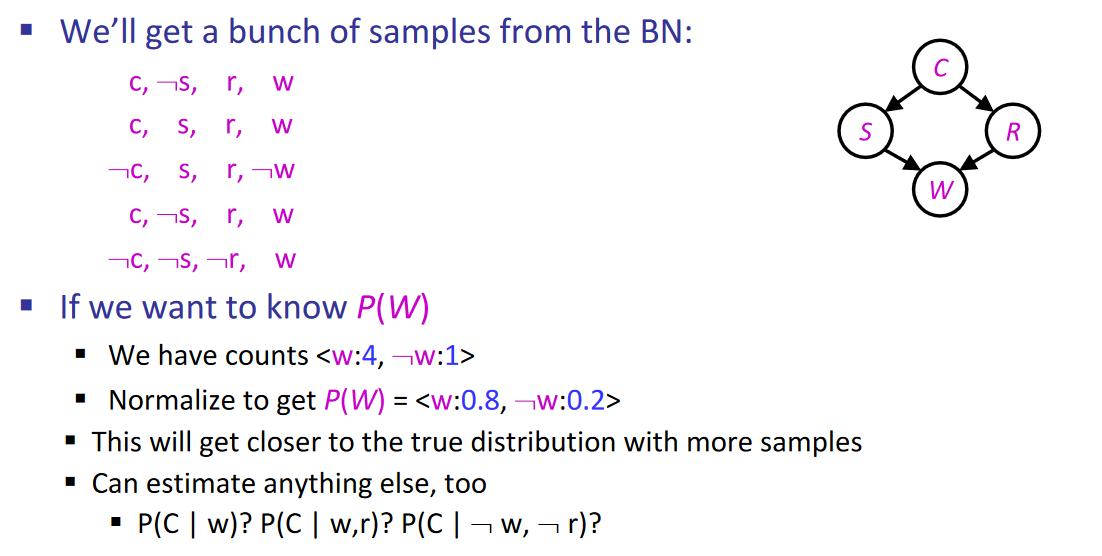
\includegraphics[width=0.6\textwidth]{pictures/priors.png}
    \end{center}
    \caption{Exemple avec Prior Sampling}\label{fig:priors}
\end{figure}


% subsubsection Prior (end)

\subsubsection{Rejection Sampling} % (fold) 
\label{sec:rejection_sampling} 

La différence avec l'échantillonage par prior est que l'on rejette les échantillons qui ne satisfont pas la condition de nos observations.

\begin{enumerate}
    \item \textbf{Initilisation}: Choisir une variable aléatoire dans le réseau bayésien.
    \item \textbf{Echantillonage}: Échantillonnez une valeur pour cette variable en utilisant sa distribution a priori. 
        Cela représente une hypothèse sur la valeur de cette variable avant de prendre en compte des observations.
    \item \textbf{Propagation}: Propagez la valeur échantillonnée dans le réseau bayésien en 
        respectant les probabilités conditionnelles définies par la structure du graphe. 
        Cela signifie que vous échantillonnez les valeurs des variables parentes en fonction des valeurs déjà échantillonnées.
        % Pour chaque variable aléatoire dans le réseau bayésien, échantillonnez une valeur en utilisant la distribution conditionnelle de cette variable étant donné les valeurs des parents de cette variable.
    \item \textbf{Rejet}: Si l'échantillon ne satisfait pas la condition, alors on le rejette.
    \item \textbf{Répétez} les étapes 2 et 3 jusqu'à ce que toutes les variables aléatoires du réseau bayésien aient une valeur échantillonnée. Ou bien jusqu'à ce que le nombre d'échantillons soit suffisant.
\end{enumerate}

\begin{example}\leavevmode
    Si nous cherchons à calculer $P(B | j, m)$, alors nous rejetons tous les échantillons qui ne satisfont pas $j$ et $m$. Car 
    on s'en fout de $\neg j$ et $\neg m$.
\end{example}

\subsubsection{Likelihood Weighting} % (fold) 
\label{sec:likelihood_weighting} 

Le problème avec l'échantillonage par rejet est que l'on rejette beaucoup d'échantillons. Si 
les données que l'ont veut sont rares, alors on va rejeter beaucoup d'échantillons et l'algorithme sera très lent.

L'idée est de générer des échantillons qui satisfont les observations. On \textbf{force} les échantillons à satisfaire les observations.
Le problème est que les échantillons ne sont plus tirés de manière aléatoire donc la distribution des échantillons n'est plus la même, elle est \textbf{biaisée}.

Pour résoudre ce problème, on va \textbf{pondérer} les échantillons avec la probabilité d'observer la variable selon ses parents.
Plus un échantillon est probable, plus il aura de poids et inversement.

\newpage
\begin{itemize}[label=\textbullet]
    \item \textbf{Input}: Les observations $E_i=e_i$. 
    \item weight $\leftarrow$ 1
    \item \textbf{Pour} chaque variable aléatoire $X_i$ dans le réseau bayésien:
        \begin{itemize}[label=\textbullet]
            \item \textbf{Si} $X_i$ est une variable observée $E_i=e_i$:
                \begin{itemize}[label=\textbullet]
                    \item $x_i \leftarrow e_i$
                    \item weight $\leftarrow$ weight $\times$ $P(X_i | Parents(X_i))$
                \end{itemize}
            \item \textbf{Sinon}:
                \begin{itemize}[label=\textbullet]
                    \item $x_i \leftarrow$ échantillon de $P(X_i | Parents(X_i))$
                \end{itemize}
        \end{itemize}
    \item \textbf{Output}: $x_1, \dots, x_n$ et weight
\end{itemize}

\begin{figure}[H]
    \begin{center}
        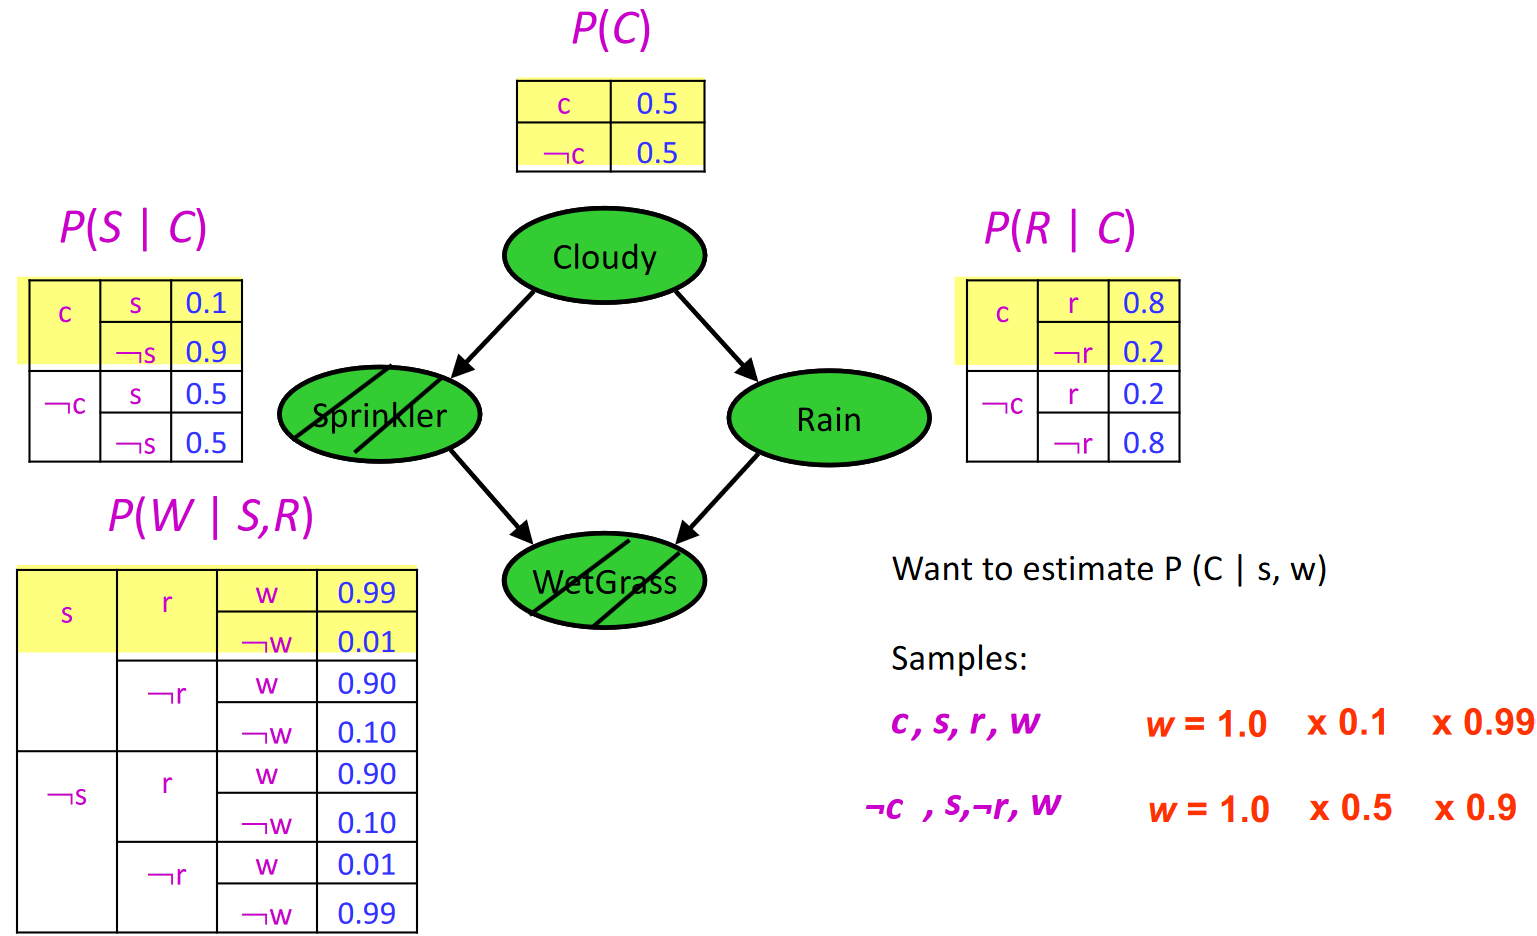
\includegraphics[width=0.55\textwidth]{pictures/likelihood.png}
    \end{center}
    \caption{Execution de Likelihood algorithme}\label{fig:likelihood}
\end{figure}

\subsubsection{Gibbs Sampling} % (fold) 
\label{sec:gibbs_sampling} 

Cette méthode résoud le problème du \textit{Likelihood Weighting} qui est qu'il risque 
d'y avoir un biais lorsque les évidences sont les variables aléatoires qui ont le plus de parents.

L'idée est de fixer les valeurs des variables observées et de générer aléatoirement des valeurs pour les autres variables. 
De cette manière, on a un échantillon de départ. Pour toutes les variables qui sont sont pas observées, on va échantillonner une valeur en fonction des valeurs des variables déjà échantillonnées tout en 
gardant les valeurs des variables observées fixes.
Chaque valeur échantillonnée est une hypothèse sur la valeur des autres variables aléatoires.

\begin{figure}[H]
    \begin{center}
        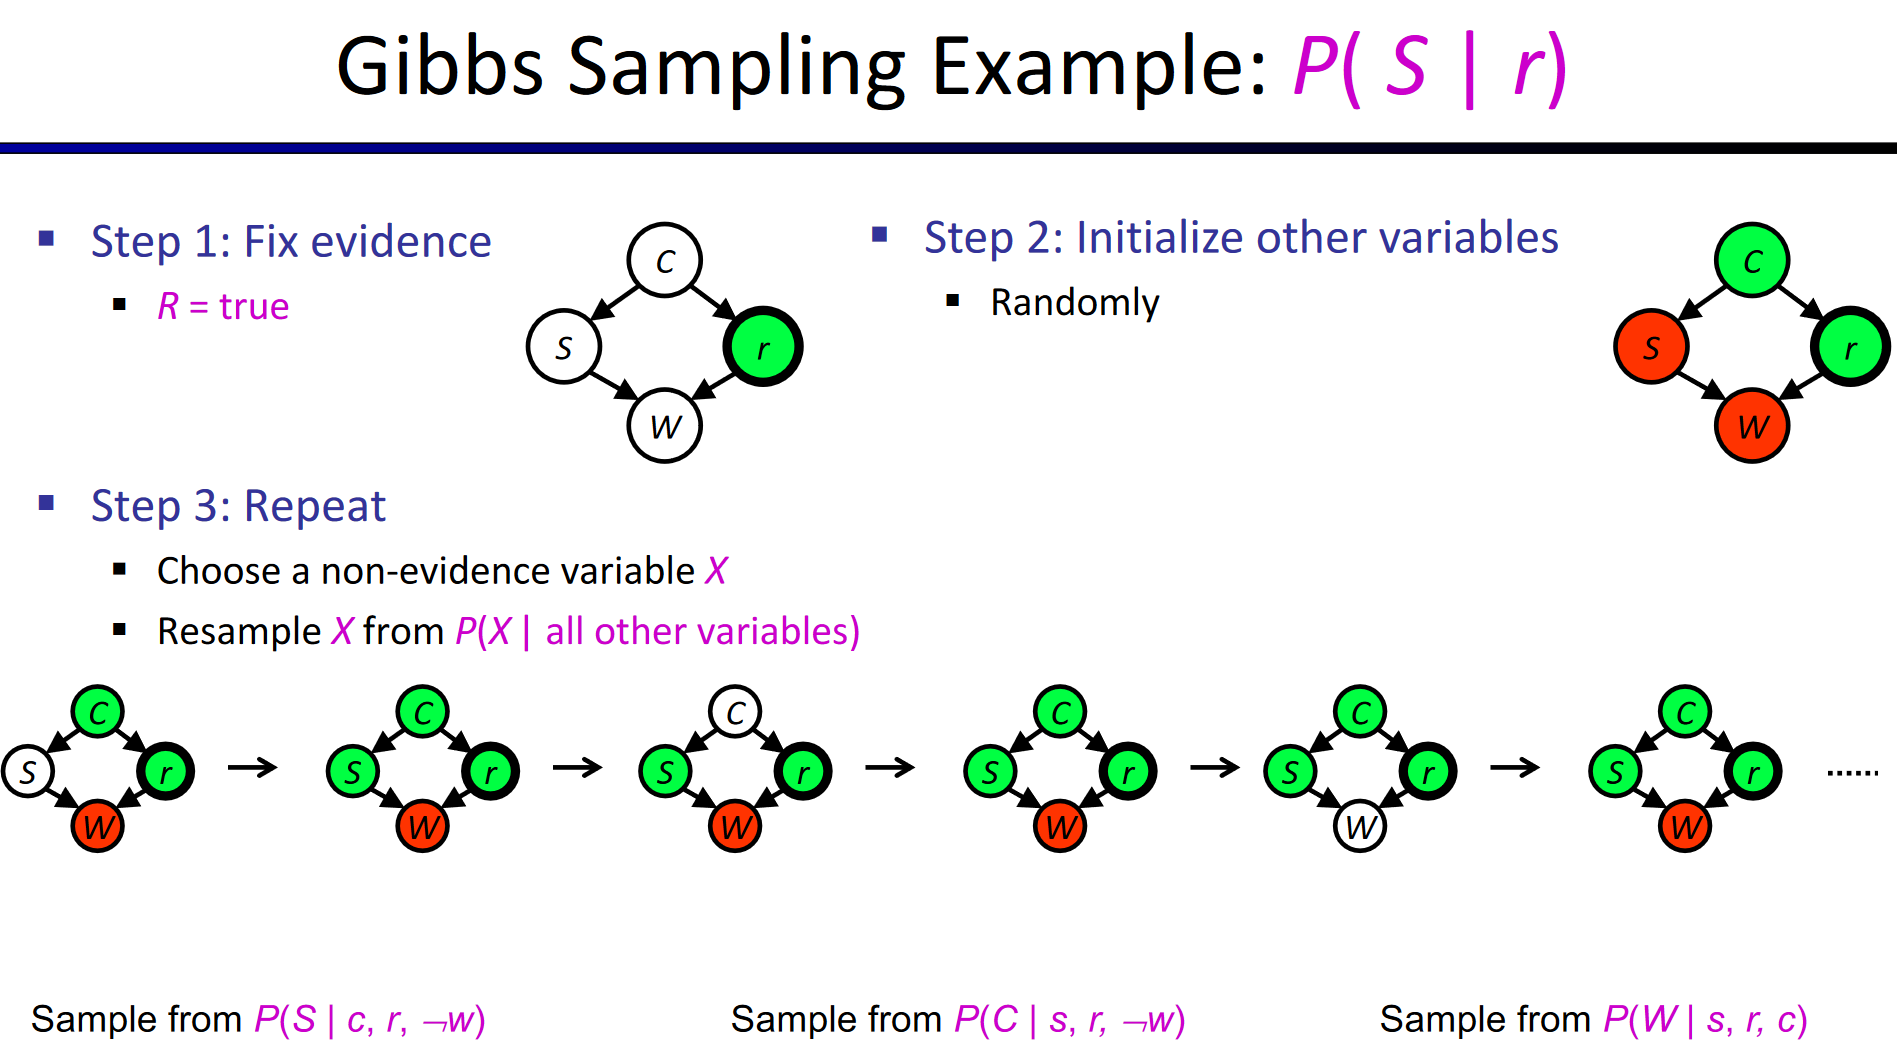
\includegraphics[width=0.5\textwidth]{pictures/gibbs.png}
    \end{center}
    \caption{Execution de l'algorithme de Gibbs}\label{fig:gibbs}
\end{figure}





% subsection Echantillonage (end)







% L'inférence par énumération se déroule en 3 étapes. 
% Nous définissons \textbf{facteurs} comme étant les tables de probabilités conditionnelles des noeuds.


% Dés qu'il y a un triplet inactif, le chemin devient inactif. S'il existe au moins un triplet actif, alors le chemin est actif.
% inactif = indépendant, actif = pas indépendant




% subsubsection Enumeration (end)



% subsection Inference (end)
